\documentclass[11pt,border=5pt]{standalone}
\usepackage{fontspec}
\setmainfont{cmunrm.otf}[BoldFont=cmunbx.otf,ItalicFont=cmunti.otf,BoldItalicFont=cmunbi.otf]
\usepackage{amsmath}
\usepackage{unicode-math}
\setmathfont{NewCMMath-Regular.otf}
\usepackage{tikz}
\usetikzlibrary{arrows.meta,patterns,angles,quotes}
\begin{document}
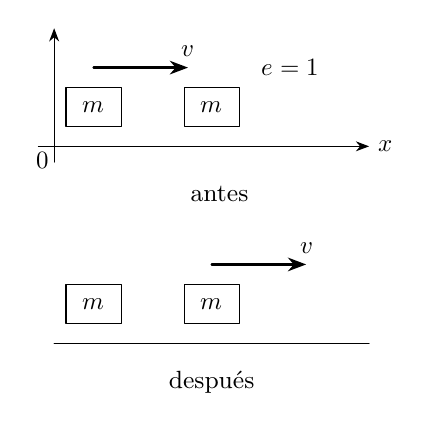
\begin{tikzpicture}[>=Stealth,font=\small,line cap=round,line join=round]
\draw[->,thin] (-0.2,0) -- (4,0) node[right] {$x$};
\draw[->,thin] (0,-0.2) -- (0,1.5);
\node at (-0.14,-0.18) {$0$};
\draw[fill=white] (0.15000000000000002,0.25) rectangle (0.85,0.75);
\node at (0.5,0.5) {$m$};
\draw[fill=white] (1.65,0.25) rectangle (2.35,0.75);
\node at (2,0.5) {$m$};
\draw[->,thick] (0.5,1) -- (1.7,1) node[above] {$v$};
\node at (3,1) {$e=1$};
\node at (2.1,-0.6) {antes};
\begin{scope}[yshift=-2.5cm]\draw[] (0,0) -- (4,0);
\draw[fill=white] (0.15000000000000002,0.25) rectangle (0.85,0.75);
\node at (0.5,0.5) {$m$};
\draw[fill=white] (1.65,0.25) rectangle (2.35,0.75);
\node at (2,0.5) {$m$};
\draw[->,thick] (2,1) -- (3.2,1) node[above] {$v$};
\node at (2,-0.5) {después};
\end{scope}
\end{tikzpicture}
\end{document}
